\documentclass{article}[12pt]

\usepackage{tikz}
\usetikzlibrary{decorations.fractals}
\usepackage{subfig}
\usepackage{natbib}
\usepackage[utf8]{inputenc}
\usepackage{amsmath}
\usepackage{url}

\widowpenalty10000
\clubpenalty10000

\newcommand{\kochstraight}[1]{
\begin{tikzpicture}[decoration=Koch snowflake]
\draw {(0,0) -- (1,0) };
\end{tikzpicture}
}

\newcommand{\kochfirst}[1]{
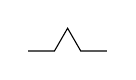
\begin{tikzpicture}[decoration=Koch snowflake]
\draw decorate{ (0,0) -- (1,0) };
\end{tikzpicture}
}

\begin{document}

\title{Fractals \\ \large Basic concepts and applications}
\author{Manuel Mezger}

\maketitle

\tableofcontents

\section{Introduction}
Some of the main questions asked by the layman, when confronted with fractal structure is "What are fractals?" or "How can calculations be performed on such seemingly random structures?" and "What are fractals good for anyway?".  The aim of this short essay is to address some of these questions by providing a brief intuitive overview on the basics of fractal theory and by then providing an example on how these methods can be used to adequately analyse empirical data, by analysing the size of German cites. At first however, a short history on the discovery of fractals shall serve as an introductory motivation to the reader.

Judging by ancient tribal art, fractal structures were already known of before he beginning of modern mathematics in ancient Greece. Although many philosophers came into contact with them, judging by their studies into naturally occurring patterns, they were often disregarded by them as being to complex or random to be captured under generalised mathematical descriptions. Following in their (questionable) footsteps, many notable mathematicians such as Gottfried Wilhelm Leibniz and Sir Isaac Newton disregarded fractal structures in their studies, for example by leaving out the analysis of fractal structures by the methods of calculus they had independently of one another discovered. It was only in the early 19th century, that under the movement of making calculus mathematically rigorous, spearheaded by the mathematicians Karl Weierstrass and Georg Cantor, fractals received some of the attention formerly reserved for easier to analyse smooth objects. It took however until the late 1960s that through his work on fractal structures, the father of the modern systematic approach towards fractal theory, Benoit Mandelbrot, finally gave fractals the widespread recognition they enjoy today \citep{falconer2013fractals}.

Nowadays methods developed through research into fractals are utilised in fields as diverse as physics, sociology, biology and economics. Using fractals, formerly hard to analyse problems such as the price development of commodities, plant growth, the overall size of regional and international conflicts, and the formation of naturally occurring lightning have become easier and more intuitive to understand \citep{liebovitch1998fractals, cioffi2013power, takayasu2000fractal}

\section{The Basics of Fractal Theory}

\subsection{The Coastline of Britain}
One oft the most common examples used to intuitively illustrate the idea of fractals is that of the "Coastline of Britain", first used by Mandelbrot himself in one of his first papers on the subject \citep{mandelbrot1967long}.

If one were to be set the task of measuring the coastline of Britain, how would be the best way to go about it? Probably the most initial thought would be to get a precise ruler and the nearest atlas at hand, and to search in it for the first map of the Island of Britain one comes across. Then one would start to measure the depicted coastline. This method would yield a first, feasible result. Turning over to the next page of the atlas however, a new map of Britain, depicted in a larger, more detailed scale comes to light. To make sure that the first measurement is correct, it seems reasonable to repeat the measuring procedure, this time taking into account all the little bays and headlands on the coast that weren't depicted on the first, more undetailed map (Figure \ref{fig:brit}). Unsurprisingly, this second measurement yields a significantly larger result, as it picks up more detail in the measuring process. This course of action could be repeated into infinitely fine scales, taking into account every pebble and grain of sand, and each time leaving us with a larger but just as ambiguous result of the definitive length of the British coast. The result that the British coastline is apparently infinite, or to say at best indeterminate, is an illustration of one of the first main concepts of fractal structures: that measurements of them rely on the scale of their resolution, in short that they are "scale-dependant" \citep{mandelbrot1967long, batty1987urban}.

The second main concept of fractal structures, that they are "self-similar", that is that details that turn apparent at a higher scaled resolution mimic the structure of details at lower scale resolutions, can also be illustrated by the British coastline. For example, the closer one looks at single large bays or headlands, the more apparent it becomes that they themselves do not form smooth objects themselves, but rather jut in and out of the sea, much like the coast of the whole island itself! This specific intuitive example of course has its real world limits, as the smallest resolution one can get to is bounded by the atomic level. Nevertheless in theory, it should be possible to scale a fractal structure into infinite detail and that by doing so one should always stumble upon similar structures that are familiar from a higher scaled level.

These two properties are the most common defining features of fractal structures. Others, such as having "details at every scale" are also, among others, commonly found in fractal structures and approximately define what a fractal is, and what isn't.
As a word of caution it should however be noted, that fractals have not yet been exclusively defined, and many structures which only show some of the defining properties can for practical purposes be regarded as being fractals.

\subsection{Stylized Fractal Structures}
Leaving our first introductory example behind us, let us now shift our attention to a more mathematically defined stylized approach towards fractal structures. One of the most simple, yet also most elegant stylized fractal structures known is that of the Koch curve, depicted in Figure \ref{fig:koch}.
The process of constructing a Koch curve is rather simple. Starting off with a straight line at the 0th step of constructing the curve, the line itself is divided into three equally long parts, with the middle section being subsequently removed and replaced by two equally long segments which connect to the two remaining sections and themselves at a 60 degree angle, forming two sides of an equilateral triangle. This process describes the steps taken to get from the starting point $E_0$ to the first step of the Koch curve generating process $E_1$ (the whole process is illustrated in Figure \ref{fig:koch_const}). To get from $E_1$ to $E_2$, or for that matter from any $E_n$ to $E_{n+1}$, the steps described for generating $E_1$ out of the$E_0$ are repeated for every segment in $E_n$ that mimic $E_0$ (in other words, every \kochstraight{} in $E_n$is replaced by a \kochfirst{} in $E_{n+1}$) (Figure \ref{fig:koch_constfull}).
This process of successively replacing similar objects at higher scales by a clearly defined function is called a Lindenmayer-system or L-system. It seems immediately apparent that structures generated by these L-systems are characterized by two of the main describing properties of fractals we have already encountered: "self-similarity" and "details at every scale".

Looking more closely at the Koch curve, we can see the pattern \kochfirst{} repeated multiple times at higher scales. Setting the size of \kochfirst{} to \kochstraight{} in relation (in our case it is $4/3$, as we replace 3 equally long segments by 4 segments with the same length) and thinking about how the measured length of the whole curve changes at every step of the generating process, we come to the conclusion that the length of the Koch curve, just like the perimeter of the coastline of Britain, cannot be measured with conventional methods and tends towards infinity. This process of thought is summarized in Table \ref{table:koch_length}.


\begin{table}[]
\begin{tabular}{p{2.5cm}ccccc}
&&&&&\\
\hline
\hline
Process step &  $E_0$ & $E_1$ & $E_2$ &  $ ... $ &$\underset{n \to \infty}{E_n} \simeq F$\\
\hline
Length of the Koch curve & $1$ & $4/3$ & $16/9$ & $ ... $ & $\infty$\\
Alternative \newline expression & $ (4/3)^0 $ & $(4/3)^1$  & $(4/3)^2$  & $...$ & $\underset{n \to \infty}{\lim}(4/3)^n$ \\
\hline
\hline
\end{tabular}
\caption{Estimating the length of the Koch curve by calculating the length of the curve at different steps of it's construction (setting the length of $E_0$ to 1)}
\label{table:koch_length}
\end{table}

It seems apparent that any other L-system, that is constructed as described in the above text, behaves in a similar fashion. This observation leaves us with the question of we have now found structures that defy any sort of conventional forms of measurement, and if we should simply give up trying the find a specific number when measuring fractal structures.

\subsection{Fractal Dimensions and Power Laws}
It is at this point we should shift our attention towards the role dimensions play in measuring the size of objects. Measurements taken on the size of objects, be it a straight line or a volume, are always dependent on the dimension we place these objects in. Most of the time, choosing the correct dimension to measure an object comes naturally to us. But imagine trying to measure the "area" taken up by a litre of water (the fluid itself, not its container) or the "area" of a drawn line (assuming no thickness). We intuitively see that choosing wrong dimensions for measuring objects leads to unhelpful, if not even wrong answers for the questions posed.
In a related manner choosing the wrong dimension for measuring fractal objects will also provide us with unhelpful answers. Until now, we have only used the one-dimensional form of measurement "length", to analyse the two examples we have until now encountered (the coastline of Britain and the Koch curve). As we have seen, it is insufficient for our analysis, as it has on both occasions provided us with un-interpretable results. Generally said, if an object possesses an infinite measure in a certain dimension, the dimension chosen might have been to small, whereas a measure of $0$ is an indicator for a too large dimension having been chosen \citep{falconer2013fractals}.

Naturally one would therefore be tempted to try sizing both structures with two-dimensional measures. It can also be shown that measuring the Koch curve or the coastline of Britain with two-dimensional measures, that is to say to measure their areas, also leaves us none the wiser (Their areas are in fact $0$, just like the area of a straight line, see \cite{falconer2013fractals}).

Judging by both structures being infinite in one dimension but non-existent in two, leaves us with the conclusion that they are too big to be thought of as one-dimensional objects, but also being too small to be thought of as two-dimensional. Their true dimension must therefore lie somewhere in between both, in a "fractional" dimension consisting of a non-integer number between one and two.
There are multiple ways to determine the fractal dimensions of a structure, each with varying complexity and detail \citep{falconer1986geometry}.As this essay is supposed to be an intuitive introduction, we will focus on one of the simplest and most straightforward for determining the dimensions of one- to two-dimensional objects: the Box-counting algorithm.
The main idea oft he algorithm can be summed up in a few words. Grids of varying box-length are laid over a structure and the number of boxes, which the structure intersects, is counted. Subsequently the result is put into proportion to the sidelength of the boxes the whole grid is composed of.
Let us look at an intuitive example of the algorithm at work. Overlaying a straight line of the length one with Grids of varying box sizes $r$, as is done in Figure \ref{fig:box_line}, and counting the number of boxes intersected by the analysed structure $N(r)$, we get Table \ref{table:box_line}.

\begin{table}[!ht]
\begin{tabular}{p{3cm}cccccc}
&&&&&&\\
\hline
\hline
Box-sidelength $r$ &  $1/4$ & $1/8$ & $1/16$ &  $1/32$ & $...$ & $r$\\
\hline
Boxes  \newline intersected $N(r)$ & $4$ & $8$ & $16$ & $32$ & $...$ & $1/r$\\
Alternative \newline expression of $N(r)$ & $ 4^1$ & $8^1$  & $16^1$  & $32^1$ & $...$ & $(1/r)^1$ \\
\hline
\hline
\end{tabular}
\caption{Estimating the dimension of a straight line with the Box-count algorithm}
\label{table:box_line}
\end{table}

It can be shown, that the number to which the inverse sidelength of the boxes used in the algorithm ($1/r$) is raised to, to equal the number of boxes intersected by the analysed structure ($N(r)$), functions as an indicator for the dimension $d$ of the object being analysed )\citep{falconer2013fractals}. Mathematically expressed, this would be equal to the expression

\begin{align}
N(r) = (1/r)^d
\label{eq:Nr}
\end{align}

In our example the power the inverse sidelengths are raised to equals $1$, which equates to:

\begin{align}
N(r) = (1/r)^1
\end{align}

This makes perfect sense, as a straight line is a one-dimensional object. Were we to lay similar grids over a square with the sidelength $1$, as is shown in Figure  \ref{fig:box_square}, we would receive Table \ref{table:box_square}.

\begin{table}[!ht]
\begin{tabular}{p{3cm}cccccc}
&&&&&&\\
\hline
\hline
Box-sidelength $r$ &  $1/4$ & $1/8$ & $1/16$ &  $1/32$ & $...$ & $r$\\
\hline
Boxes  \newline intersected $N(r)$  & $16$ & $64$ & $256$ & $1024$ & $...$ & $1/r^2$\\
Alternative \newline expression of $N(r)$ & $ 4^2$ & $8^2$  & $16^2$  & $32^2$ & $...$ & $(1/r)^2$ \\
\hline
\hline
\end{tabular}
\caption{Estimating the dimension of a square with the Box-count algorithm}
\label{table:box_square}
\end{table}

We see immediately that, as expected, the exponent in the second row equals $2$, which leads to the equation 

\begin{align}
N(r) = (1/r)^2
\end{align}

As a square is a two-dimensional object, Table \ref{table:box_square} can be seen as a further illustration of the validity of Equation \ref{eq:Nr}.

Let us now turn our attention back to the more interesting case of the Koch curve. The Box-counting algorithm provides us with an easy way of identifying its dimension, which until now has been unknown. Just as with a straight line or a square, we lay ever finer structured grids over the Koch curve and count the number of intersected boxes (Figure \ref{fig:box_koch}). The results we get are shown in Table \ref{table:box_koch}.

\begin{table}[!ht]
\begin{tabular}{p{3cm}cccccc}
&&&&&&\\
\hline
\hline
Box-sidelength $r$ &  $1/4$ & $1/8$ & $1/16$ &  $1/32$ & $...$ & $r$\\
\hline
Boxes  \newline intersected $N(r)$  & $6$ & $14$ & $33$ & $78$ & $...$ & $1/r^{1.2618}$\\
Alternative \newline expression of $N(r)$ & $ 4^{1.292}$ & $8^{1.269}$  & $16^{1.2619}$  & $32^{1.257}$ & $...$ & $(1/r)^{1.218}$ \\
\hline
\hline
\end{tabular}
\caption{Estimating the dimension of the Koch curve the Box-count algorithm}
\label{table:box_koch}
\end{table}

From Table \ref{table:box_koch} we can gather that that, with a decreasing sidelength $r$, the exponent we raise $1/r$ to, to equal $N(r)$ converges approximately against $1.2618$. This indicates that the Koch curve is approximately a 1.26-dimensional object with the approximate estimation function for the number of intersected boxes

\begin{align}
N(r) = (1/r)^{1.26}
\end{align}

At this point we should note that until now we have only performed box-counting on objects normalized to a length or an area of $1$. Were we to vary the size of our objects and determine Equation \ref{eq:Nr} to estimate the number of boxes counted, as we did before, we would receive Table \ref{table:box_const}.


\begin{table}[!ht]
\begin{tabular}{p{5cm}c}
&\\
\hline
\hline
Line segment of length 2 & $N(r)=2(1/r)^1$ \\[2.5ex]
\hline
Line segment of length 3 & $N(r)=3(1/r)^1$ \\[2.5ex]
\hline
Square of length 2 & $N(r)=4(1/r)^2$ \\[2.5ex]
\hline
Square of length 3 & $N(r)=9(1/r)^2$ \\[2.5ex]
\hline
\hline
\end{tabular}
\caption{Effect of varying the size of objects analysed by the Box-counting algorithm on the number of boxes counted}
\label{table:box_const}
\end{table}

Before proceeding should therefore generalise Equation \ref{eq:Nr} by adding a constant $c$ to the expression 

\begin{align}
N(r) = c(1/r)^d
\label{eq:pow}
\end{align}

This Equation is also known as a power law, as the number $(1/r)$ is consistently raised by the fixed power of $d$. In it the variables $c$ and $d$ are also known as the multiplier and the exponent (respectively), and characterise the function.
Say we wanted to generalise the process of computing our exponent $d$ from a given structure. By taking logarithms on both sides of Equation \ref{eq:pow}, we would receive the equation

\begin{align}
log(N(r)) = log(c(1/r)^d)
= log(c) + log(1/r)d
\label{eq:d_comp}
\end{align}

which can, by the use of simple algebra, be written as

\begin{align}
\frac{log(N(r))}{log(1/r)} = \frac{log(c)}{log(1/r)}+d
\end{align}

which can be transformed to

\begin{align}
d = \frac{log(N(r))}{log(1/r)} - \frac{log(c)}{log(1/r)} \underset{r \to 0}{\simeq} \frac{log(N(r))}{log(1/r)}
\end{align}

as $log(1/r)$ will grow increasingly larger as $r$ gets infinitely small whereas $log(c)$ remains constant. 

Having now roughly given an overview over the idea of fractal dimensions and power laws, it is time to apply our newly gained theoretical knowledge on real world data.

\section{Power Law Distributions in German City Sizes}
\subsection{Previous Research}

Due to increased trends in urbanisation in developed and especially in developing countries, the distribution of the sizes of urban centres has in the past already been the subject of a great amount of research \citep{chen2003rank, arcaute2015constructing, batty1987urban}. As they tend to grow at exponential rates, research on the fractional structure of city sizes has been at the forefront of this new branch of urban studies. Nowadays, through empirical work conducted on cities in the United States, Great Britain and China, it is common consensus that city sizes follow a power law distribution, and are uniformly characterized by slightly differing fractal structures \citep{newman2005power, batty1987urban}. Thinking back to the definitions of fractal structures we got to know discussing the coastline of Britain, this observation seems intuitive. Breaking large cities up into smaller parts like administrative districts of boroughs, we can see similar structures that characterised the large city as a whole, like city centres, parks or main streets, mimicked by these smaller fragments. The aim of this last part of this essay is therefore to apply the methods we discussed to analyse the distribution of German city sizes, and compute their fractal dimension. 

\subsection{Empirical Results}
The data for the German city sizes was scraped from the website \newline \scriptsize \url{https://de.wikipedia.org/wiki/Liste_der_Gro%C3%9F_und_Mittelst%C3%A4dte_in_Deutschland}, \newline \normalsize which itself sourced its data directly from the Statistisches Bundesamt, the German federal office for statistics.

Going off on a Tangent, the advantage of using the method of scrapping data directly from websites, as opposed to getting it as datasets from official institutes, is that the research performed is immediately reproducible for anyone with and an internet connection and the necessary programs installed necessary to run the code used, without having to exchange datasets. To get a feel for the being used in this essay, I would therefore ask you to feel free to run the script provided with it.

But lets go back to the data at hand. Plotting the size of German cities in a histogram shows us that the data follows a right skewed distribution with a pronounced fat tail going towards the right (Figure \ref{fig:city_hist}). This is a strong visual indicator for a data following a power law \citep{newman2005power}. Using Equation \ref{eq:pow}, we should be able to estimate that the count for the number of cities of a certain size $s$ in Germany, denoted by the shorthand $N(s)$, by the equation

\begin{align}
N(s) = c(s)^{-d}
\label{eq:city}
\end{align}

A quick visual check if we are correct in our assumption can be found in Figure \ref{fig:city_plot}. If the distribution does indeed follow a power law, a plot of the logged count of the number of cities $N(s)$ of certain size $s$ onto the logarithm of that size $s$ should roughly follow a downward sloping line with the gradient $-d$, as the following Equation shows

\begin{align}
log(N(s)) = -d \cdot log(s)
\label{eq:d_slope}
\end{align}

As Figure \ref{fig:city_plot} shows, we can indeed make out a linear trend. The growing fluctuations at the bottom of the graph as the counts get smaller and the city sizes get higher, should mainly be considered as statistical fluctuations in the data set, due to smaller variations in the count have stronger impacts on deviations from the trend, and not necessarily as a contradiction to the hypothesis of a power law distribution \citep{newman2005power}.

Thinking back to Equation \ref{eq:est_d} and using basic algebra, we might come to the conclusion that an efficient way of estimating the dimension of the city sizes $d$ is given by the equation

\begin{align}
-d =  \frac{log(N(s))}{log(s)}
\label{eq:est_d}
\end{align}


The avid statistician might now feel inclined to use a simple OLS-Estimation on the data presented in Figure \ref{fig:city_plot}, to get the best estimate for the value of $d$. This approach has been used sporadically in previous research such as \cite{cioffi2013power} and \cite{ takayasu2000fractal}, other researchers such as \cite{clauset2009power}and \cite{newman2005power} were however successful in showing that a Maximum likelihood estimate (MLE) early always provides better results. Both argue that differences that arise in both estimation techniques come down to a different treatment of the statistical fluctuations we have already encountered in Figure \ref{fig:city_plot}. Using the notation we are already familiar with, the ML-estimator described by the latter for structures larger than one-dimension can be expressed as

\begin{align}
d = 1+ n\left[  \sum\limits_{i} log \frac{x_i}{x_{min}}  \right]^{-1}
\label{eq:d_mle}
\end{align}

where $x_min$ describes the threshold at which our data ceases to show "self-similarity" and "details at every scale" (in our case the smallest city in our dataset with 20.040 inhabitants), $x_i$ stands for every data point in our distribution (in our case every German city with more than 20.000 inhabitants) and $n$ describes the number of data points collected (in our case $678$ cities). For a detailed derivation of Equation \ref{eq:d_mle} please see \cite{newman2005power}.

Running our data through the ML-estimator gives us estimated value of $d$ at $2.347$. A Comparison to similar studies conducted on city sizes in other parts of the world can be found in Table \ref{table:box_const}.

\begin{table}[!ht]
\begin{tabular}{p{1.75cm}cccc}
&\\
\hline
\hline
Country & USA & UK & China & Germany \\[2.5ex]
\hline
Estimated \newline dimension & $2.30$ & $2.07$ & $[1.8241, 2.2975]$ & $2.347$
\\[2.5ex]
Source & \scriptsize \cite{ newman2005power} & \scriptsize \cite{arcaute2015constructing} & \scriptsize \cite{ gangopadhyay2009city} & -\\[2.5ex]
\hline
\hline
\end{tabular}
\caption{Comparison of the dimension $d$ of cities in different countries}
\label{table:box_const}
\end{table}


From it we can conclude, that German cities, just like their counterparts in China, the US and the United Kingdom develop roughly in similar fractal structures. Differences in the exponents could be traced back to stark divergences in urban trends, such as in the case of London in the United Kingdom, or to different statuses of growth and development, as can be seen in China. To analyse these differences, is the work of further research.

\section{Conclusion}

The aim of this short essay was to provide a basic introduction into the field of fractal theory and to show how its results can be applied to real world phenomena. It should however be noted, that it by no way understands itself as a thorough discussion of all the concepts referenced by it, but rather as a rough sketch of what is possible when applying fractal theory.

That being said, ever since Mandelbrot began publishing his first papers in the late 60s, fractal theory has opened up completely new worlds to scientific researchers, providing them with new ways to analyse complex structures. It is now up to upcoming researchers, to identify patterns in their fields, which have until now defied traditional research, and test whether they might be analysable using fractal theory. It is therefore paramount, that nowadays every empirical researcher, even if he doesn't plan on diving to deeply into theoretical mathematics, has a rough idea of what is possible in the fascinating world of fractals.


\clearpage
% Figures
\section{Figures}

\begin{figure}[!h]
    \centering
    \subfloat[Map of the British Isles at a smaller scale]{{\includegraphics[width=5cm]{BC_undet} }}%
    \qquad
    \subfloat[Map of the British Isles at a larger scale]{{\includegraphics[width=5cm]{BC_det} }}%
    \caption{Illustration of the impact of scaling on the details of a map of the British Isles}%
    \label{fig:brit}%
\end{figure}

\begin{figure}
 \centering
 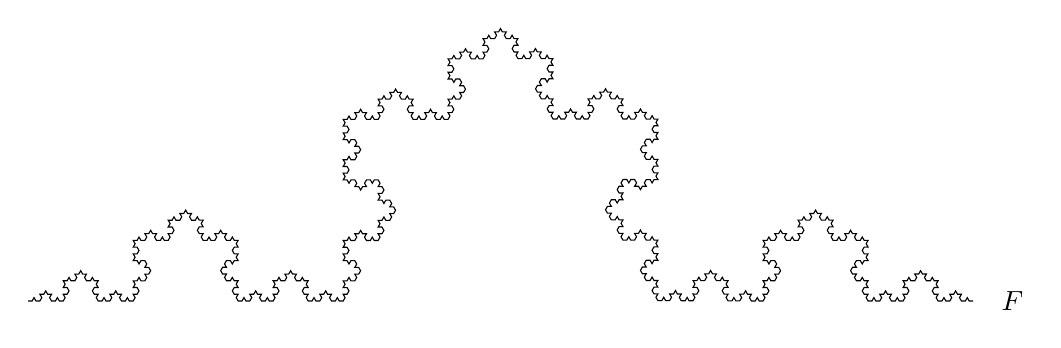
\begin{tikzpicture}[decoration=Koch snowflake]
  \draw decorate{decorate{ decorate{ decorate{ decorate{{(0,0) -- (12,0) }}}}}};
  \node at (12.5,0) {$F$};
 \end{tikzpicture}
  \caption{A detailed Koch curve}
  \label{fig:koch}%
\end{figure}

\begin{figure}
{\centering

\begin{tikzpicture}[decoration=Koch snowflake]
\draw {(0,0) -- (5,0) };
\node at (5.5,0) {$(a)$};
\end{tikzpicture}

\begin{tikzpicture}[decoration=Koch snowflake]
\node at (4.15,0) {$\downarrow$};
\node at (5,0) {$\:$};
\end{tikzpicture}

\begin{tikzpicture}[decoration=Koch snowflake]
\draw {(0,0) -- (5,0) };
\draw {(5/3,0.1) -- (5/3,-0.1) };
\draw {(10/3,0.1) -- (10/3,-0.1) };
\node at (5.5,0) {$(b)$};
\end{tikzpicture}

\begin{tikzpicture}[decoration=Koch snowflake]
\node at (4.15,0) {$\downarrow$};
\node at (5,0) {$\:$};
\end{tikzpicture}

\begin{tikzpicture}[decoration=Koch snowflake]
\draw {(0,0) -- (5/3,0) };
\draw {(10/3,0) -- (5,0) };
\node at (5.5,0) {$(c)$};
\end{tikzpicture}

\begin{tikzpicture}[decoration=Koch snowflake]
\node at (4.15,0) {$\downarrow$};
\node at (5,0) {$\:$};
\end{tikzpicture}

\begin{tikzpicture}[decoration=Koch snowflake]
\draw decorate{ (0,0) -- (5,0) };
\node at (5.5,0) {$(d)$};
\end{tikzpicture}

}
\caption{The basic process of constructing a Koch curve}
  \label{fig:koch_const}
\end{figure}

\begin{figure}
{\centering
\vbox{
\begin{tikzpicture}[decoration=Koch snowflake]
\draw {(0,0) -- (5,0) };
\node at (5.5,0) {$E_0$};
\end{tikzpicture}

\begin{tikzpicture}[decoration=Koch snowflake]
\draw decorate{ (0,0) -- (5,0) };
\node at (5.5,0) {$E_1$};
\end{tikzpicture}

\begin{tikzpicture}[decoration=Koch snowflake]
\draw decorate{ decorate{ (0,0) -- (5,0) }};
\node at (5.5,0) {$E_2$};
\end{tikzpicture}

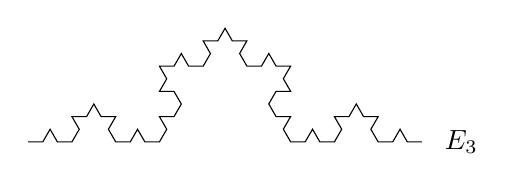
\begin{tikzpicture}[decoration=Koch snowflake]
\draw decorate{ decorate{ decorate{ (0,0) -- (5,0) }}};
\node at (5.5,0) {$E_3$};
\end{tikzpicture} \\}

\begin{tikzpicture}[decoration=Koch snowflake]
\node at (4.25,0) {$\vdots$};
\node at (5,0) {$\:$};
\end{tikzpicture}

{\centering
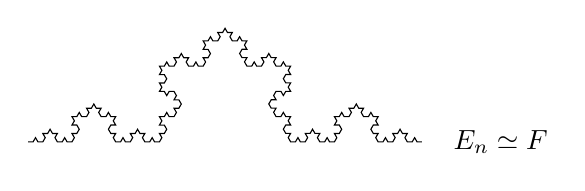
\begin{tikzpicture}[decoration=Koch snowflake]
\draw decorate{ decorate{ decorate{ decorate{ (0,0) -- (5,0) }}}};
\node at (6,0) {$E_n  \simeq F$};
\end{tikzpicture}\\}
}
\caption{The steps of constructing a full Koch curve from $E_0$ to $F$}
  \label{fig:koch_constfull}
\end{figure}

\begin{figure}[!h]
    \centering
    \subfloat[A straight line overlayed with a boxgrid of the sidelength $1/4$]{{
    
    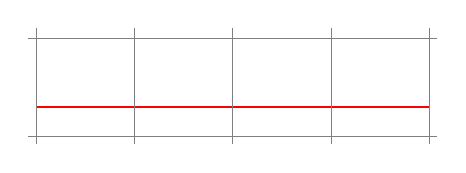
\begin{tikzpicture}[decoration=Koch snowflake, scale=0.5]
    \draw[red,thick] {(0,0.75) -- (10,0.75)};
    \draw[step = 2.5, style=help lines] (-0.2,-0.2) grid (10.2,2.75);
    \end{tikzpicture}
    
     }}%
    \qquad
    \subfloat[A straight line overlayed with a boxgrid of the sidelength $1/8$]{{
    
    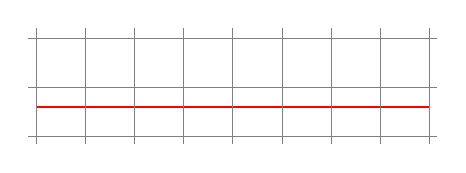
\begin{tikzpicture}[decoration=Koch snowflake, scale=0.5]
    \draw[red,thick] {(0,0.75) -- (10,0.75)};
    \draw[step = 1.25, style=help lines] (-0.2,-0.2) grid (10.2,2.75);
    \end{tikzpicture}
    
     }}%
    \qquad
    \subfloat[A straight line overlayed with a boxgrid of the sidelength $1/16$]{{
    
    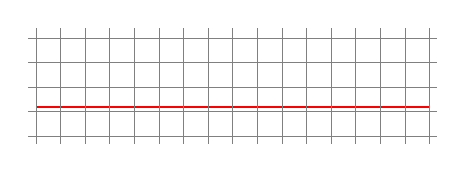
\begin{tikzpicture}[decoration=Koch snowflake, scale=0.5]
    \draw[red,thick] {(0,0.75) -- (10,0.75)};
    \draw[step = 0.625, style=help lines] (-0.2,-0.2) grid (10.2,2.75);
    \end{tikzpicture}
    
     }}%
    \qquad
    \subfloat[A straight line overlayed with a boxgrid of the sidelength $1/32$]{{
    
    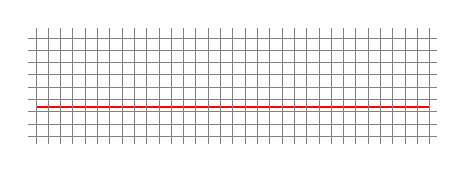
\begin{tikzpicture}[decoration=Koch snowflake, scale=0.5]
    \draw[red,thick] {(0,0.75) -- (10,0.75)};
    \draw[step = 0.3125, style=help lines] (-0.2,-0.2) grid (10.2,2.75);
    \end{tikzpicture}
    
     }}%
    \caption{Application of the Box-counting algorithm on straight line (filled red, length $1$) with varying box-sidelengths}%
    \label{fig:box_line}%
\end{figure}

\begin{figure}[!h]
    \centering
    \subfloat[Square overlayed with a boxgrid of the sidelength $1/4$]{{
    
    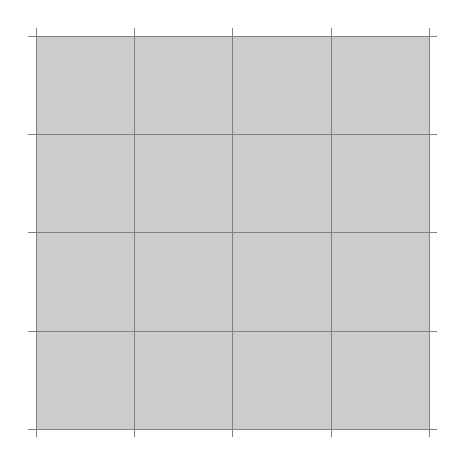
\begin{tikzpicture}[decoration=Koch snowflake, scale=0.5]
    \fill[gray!40!white] (0,0) rectangle (10,10);
    \draw[step = 2.5, style=help lines] (-0.2,-0.2) grid (10.2,10.2);
    \end{tikzpicture}
    
     }}%
    \qquad
    \subfloat[Square overlayed with a boxgrid of the sidelength $1/8$]{{
    
    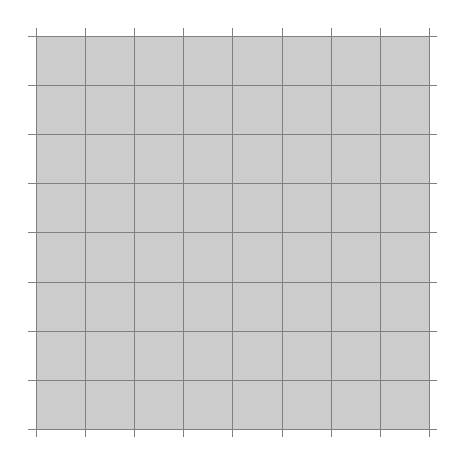
\begin{tikzpicture}[decoration=Koch snowflake, scale=0.5]
    \fill[gray!40!white] (0,0) rectangle (10,10);
    \draw[step = 1.25, style=help lines] (-0.2,-0.2) grid (10.2,10.2);
    \end{tikzpicture}
    
     }}%
    \qquad
    \subfloat[Square overlayed with a boxgrid of the sidelength $1/16$]{{
    
    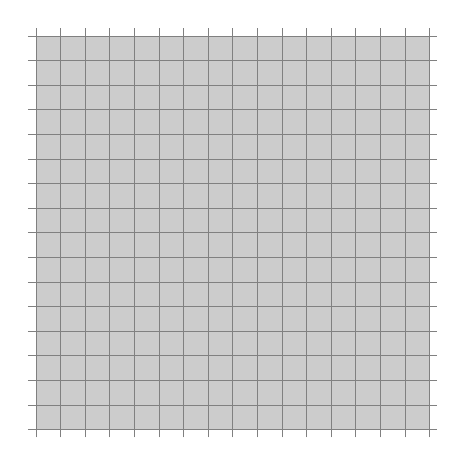
\begin{tikzpicture}[decoration=Koch snowflake, scale=0.5]
    \fill[gray!40!white] (0,0) rectangle (10,10);
    \draw[step = 0.625, style=help lines] (-0.2,-0.2) grid (10.2,10.2);
    \end{tikzpicture}
    
     }}%
    \qquad
    \subfloat[Square overlayed with a boxgrid of the sidelength $1/32$]{{
    
    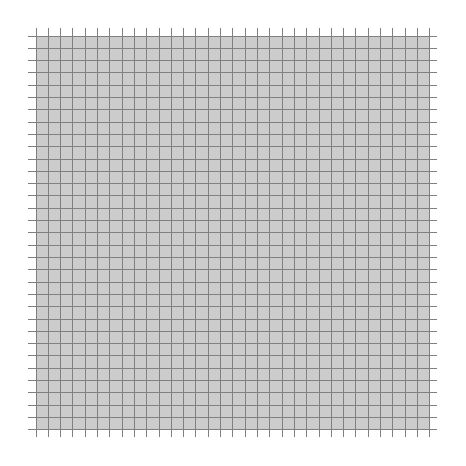
\begin{tikzpicture}[decoration=Koch snowflake, scale=0.5]
    \fill[gray!40!white] (0,0) rectangle (10,10);
    \draw[step = 0.3125, style=help lines] (-0.2,-0.2) grid (10.2,10.2);
    \end{tikzpicture}
    
     }}%
    \caption{Application of the Box-counting algorithm on a square (filled grey, sidelength $1$) with varying box-sidelengths}%
    \label{fig:box_square}%
\end{figure}

\begin{figure}[!h]
    \centering
    \subfloat[Koch curve overlayed with a boxgrid of the sidelength $1/4$]{{
    
    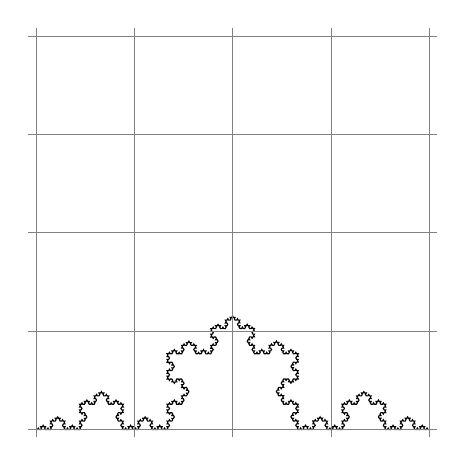
\begin{tikzpicture}[decoration=Koch snowflake, scale=0.5]
    \draw decorate{decorate{ decorate{ decorate{ decorate{{(0,0) -- (10,0) }}}}}};
    \draw[step = 2.5, style=help lines] (-0.2,-0.2) grid (10.2,10.2);
    \end{tikzpicture}
    
     }}%
    \qquad
    \subfloat[Koch curve overlayed with a boxgrid of the sidelength $1/8$]{{
    
    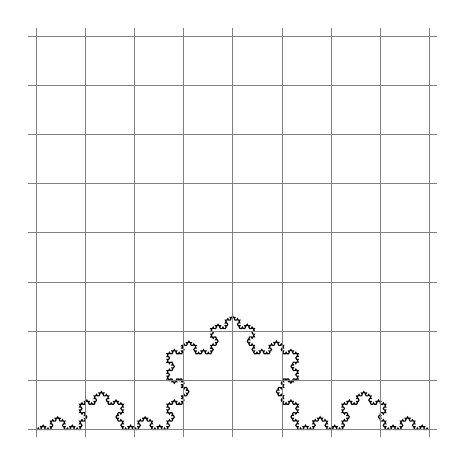
\begin{tikzpicture}[decoration=Koch snowflake, scale=0.5]
    \draw decorate{decorate{ decorate{ decorate{ decorate{{(0,0) -- (10,0) }}}}}};
    \draw[step = 1.25, style=help lines] (-0.2,-0.2) grid (10.2,10.2);
    \end{tikzpicture}
    
     }}%
    \qquad
    \subfloat[Koch curve overlayed with a boxgrid of the sidelength $1/16$]{{
    
    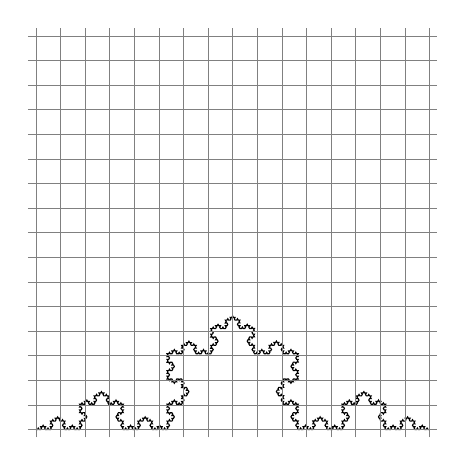
\begin{tikzpicture}[decoration=Koch snowflake, scale=0.5]
    \draw decorate{decorate{ decorate{ decorate{ decorate{{(0,0) -- (10,0) }}}}}};
    \draw[step = 0.625, style=help lines] (-0.2,-0.2) grid (10.2,10.2);
    \end{tikzpicture}
    
     }}%
    \qquad
    \subfloat[Koch curve overlayed with a boxgrid of the sidelength $1/32$]{{
    
    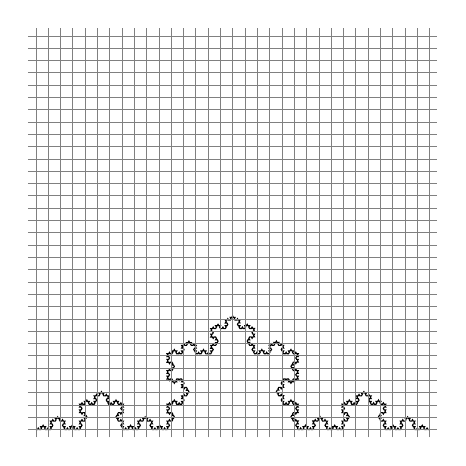
\begin{tikzpicture}[decoration=Koch snowflake, scale=0.5]
    \draw decorate{decorate{ decorate{ decorate{ decorate{{(0,0) -- (10,0) }}}}}};
    \draw[step = 0.3125, style=help lines] (-0.2,-0.2) grid (10.2,10.2);
    \end{tikzpicture}
    
     }}%
    \caption{Application of the Box-counting algorithm on the Koch curve, constructed from an $E_0$ of length $1$, with varying box-sidelengths}%
    \label{fig:box_koch}%
\end{figure}

\begin{figure}[!h]
    \centering
    \includegraphics[width=10cm]{city_hist}%
    \caption{Histogram of German city sizes}%
    \label{fig:city_hist}%
\end{figure}

\begin{figure}[!h]
    \centering
    \includegraphics[width=10cm]{city_plot}%
    \caption{Log-Log-Scatterplot of the number cities in Germany at a given city size}%
    \label{fig:city_plot}%
\end{figure}

\clearpage

\addcontentsline{toc}{section}{References} 
\bibliographystyle{chicago}
\bibliography{Bib}

\end{document}